\chapter{Theoretical Background}
\label{Chapter3}
\lhead{Chapter 3. \emph{Theoretical Background}} % Write in your own chapter title to set the page header
In our research, we have studied several key papers in the field of Natural Language Processing (NLP) to gain insights into pretraining, fine-tuning strategies, and sentence embeddings. The techniques that we will discuss in this chapter have been taken from some important research papers.
\section{SMART: Smoothness Inducing Adversarial Regularization and Bregman Proximal Point Optimization: Rooshan Khan}
\label{sec:SMART_theory}
This framework was introduced in the research paper \textit{SMART: Robust and Efficient Fine-Tuning for Pre-trained Natural Language Models through Principled Regularized Optimization} by Jiang et al. \cite{jiang2019smart}
Aggressive fine-tuning often causes the model to overfit the training data of downstream tasks, resulting in poor generalization to unseen data. To tackle this problem, the authors introduced a novel learning framework aimed at improving generalization performance.

\subsection{Framework Overview}

The proposed framework consists of two fundamental techniques to enhance the fine-tuning process of pre-trained language models:

\begin{enumerate}
  \item \textbf{Smoothness-Inducing Adversarial Regularization:} \\[0.5em]
  This technique enforces local smoothness by penalizing the model's sensitivity to small input perturbations. Specifically, it identifies the worst-case perturbation within an $\epsilon$-ball around each input. First, for each sample \( x_i \), we find a nearby perturbed input \( \tilde{x}_i \) that maximizes the smoothness loss. Then, we minimize the combined task and smoothness loss over model parameters \( \theta \).  A symmetrized Kullback-Leibler divergence is applied for classification tasks, while a squared loss is used for regression. This regularization effectively controls the model complexity and mitigates overfitting. The mathematics of this technique can be understood from the equations given below. We solve the following optimization for fine-tuning.
    \[
    \min_{\theta} \mathcal{F}(\theta) = \mathcal{L}(\theta) + \lambda_s \mathcal{R}_s(\theta),
    \]
    where $\mathcal{L}(\theta)$ represents the loss function which is defined as

    \[
    \mathcal{L}(\theta) = \frac{1}{n} \sum_{i=1}^{n} \ell(f(x_i; \theta), y_i),
    \]

    and $\ell(\cdot, \cdot)$ denotes the task-specific loss function (We used Binary Cross Entropy loss function for Paraphrase Detection, MSE loss function for STS, and Cross Entropy loss function for Sentiment Analysis), $\lambda_s > 0$ is a tuning parameter, and $\mathcal{R}_s(\theta)$ is the Smoothness-Inducing Adversarial Regularizer. Here we define $\mathcal{R}_s(\theta)$ as

    \[
    \mathcal{R}_s(\theta) = \frac{1}{n} \sum_{i=1}^{n} \max_{\|\tilde{x}_i - x_i\|_p \leq \epsilon} \ell_s(f(\tilde{x}_i; \theta), f(x_i; \theta)),
    \]

    where $\epsilon > 0$ is a tuning parameter. Note that for classification tasks, $f(\cdot; \theta)$ outputs a probability simplex\footnote{For \( n \) possible outcomes, a point in the probability simplex is a vector \( \mathbf{p} = (p_1, p_2, \dots, p_n) \), where \( p_i \geq 0 \) for all \( i \), and \( \sum_{i=1}^{n} p_i = 1 \).} and $\ell_s$ is chosen as the symmetrized KL-divergence, i.e.,

    \[
    \ell_s(P, Q) = \mathcal{D}_{\mathrm{KL}}(P \| Q) + \mathcal{D}_{\mathrm{KL}}(Q \| P);
    \]
    KL Divergence has the following formula:
    \[
    D_{\mathrm{KL}}(P \parallel Q) = \sum_{x \in \mathcal{X}} P(x) \log \left( \frac{P(x)}{Q(x)} \right)
    \]
    For regression tasks, $f(\cdot; \theta)$ outputs a scalar and $\ell_s$ is chosen as the squared loss, i.e.,
    \[
    \ell_s(p, q) = (p - q)^2.
    \]

  \item \textbf{Bregman Proximal Point Optimization:} \\[0.5em]
  To stabilize fine-tuning, this method adds a penalty based on a Bregman divergence that constrains parameter updates. It ensures that each update remains close to the previous parameters, thereby preventing excessively aggressive changes. A momentum variant further accelerates convergence and enhances stability.
  The equations related to this technique are given below. At the (t+1)-th iteration, the Vanilla Bregman Proximal Point (VBPP) method takes
    \[
    \theta_{t+1} = \arg\min_{\theta} \mathcal{F}(\theta) + \mu D_{\mathrm{Breg}}(\theta, \theta_t)
    \]
    where $\mu>0$ and the Bregman Divergence is given by
    \[
    D_{\mathrm{Breg}}(\theta, \theta_t) = \frac{1}{n} \sum_{i=1}^n \ell(f(\theta; x_i), f(\theta_t; x_i))
    \]
    In our implementation we have acceleration by momemtum as well so our parameters get updated like this:
    \[
    \theta_{t+1} = \arg\min_{\theta} \mathcal{F}(\theta) + \mu D_{\mathrm{Breg}}(\theta, \tilde{\theta}_t)
    \]
    where
    \[
    \tilde{\theta}_t = (1 - \beta) \theta_t + \beta \theta_{t-1}
    \]
    is the exponential moving average and $\beta \in (0, 1)$ is the momentum parameter. This is  the momentum Bregman proximal point (MBPP)
    method.

\subsection{Implementation of SMART}

We implemented the SMART algorithm on all three tasks. We observed improvements in the accuracies of all the tasks (Sentiment Analysis, Semantic Textual Similarity, and Paraphrase Detection). We also observed that the maximum accuracy is now achieved in fewer epochs. However, the drawbacks are that the time required to train each epoch has increased by 4 to 5 times compared to training without SMART, and additional memory is required. Specifically, for the Paraphrase Detection task, each epoch now takes approximately 5 hours with SMART, compared to 50 minutes without SMART.

\end{enumerate}
\section{Mathematical Foundations and Intuition Behind Supervised SimCSE Contrastive Loss: Abdul Samad}
\subsection{Introduction}
SimCSE (Simple Contrastive Learning of Sentence Embeddings) is a powerful technique for learning sentence representations that capture semantic meaning. This technique was introduced in the reserach paper \textit{SimCSE: Simple Contrastive Learning of Sentence Embeddings} by Gao et al.~\cite{gao2021simcse}. This document explains in depth the mathematics and intuition behind the Supervised SimCSE approach and its adaptation to paraphrase detection, especially in the context of the SNLI dataset. The goal is to enable anyone with basic machine learning understanding to grasp the core concepts.

\subsection{Why Contrastive Learning?}

In traditional classification, we teach models to map inputs to fixed class labels. In contrastive learning, we teach models to understand relationships between inputs, especially:
\begin{itemize}
    \item Which examples should be close (positive pairs)
    \item Which examples should be far apart (negative pairs)
\end{itemize}

We do this by pulling similar sentence embeddings together and pushing dissimilar ones apart. The result is a semantic embedding space where cosine similarity reflects actual meaning.

\subsection{Sentence Embeddings and Similarity}

Given a sentence, BERT produces a high-dimensional vector (embedding). To compare two sentences:
\begin{enumerate}
    \item Convert both into vectors (via BERT and pooling)
    \item Normalize the vectors
    \item Measure cosine similarity:
\end{enumerate}

\[
\text{sim}(\mathbf{u}, \mathbf{v}) = \frac{\mathbf{u}^\top \mathbf{v}}{\|\mathbf{u}\| \cdot \|\mathbf{v}\|}
\]

If vectors are unit-normalized:

\[
\text{sim}(\mathbf{u}, \mathbf{v}) = \mathbf{u}^\top \mathbf{v}
\]

\subsection{Supervised SimCSE Using SNLI Triplets}

\subsubsection{Dataset Structure}

Each training example is a triplet:
\begin{itemize}
    \item Anchor ($a$): Premise
    \item Positive ($p$): Hypothesis with entailment
    \item Negative ($n$): Hypothesis with contradiction
\end{itemize}

\subsubsection{Goal}

We want:
\begin{itemize}
    \item The similarity between $a$ and $p$ to be high
    \item The similarity between $a$ and $n$ to be low
\end{itemize}

\subsubsection{Mathematical Loss Derivation}

Let:
\begin{itemize}
    \item $\mathbf{a}_i$: embedding of anchor
    \item $\mathbf{p}_i$: embedding of positive
    \item $\mathbf{n}_i$: embedding of negative
\end{itemize}

All embeddings are L2-normalized:

\[
s^+_i = \mathbf{a}_i^\top \mathbf{p}_i, \quad s^-_i = \mathbf{a}_i^\top \mathbf{n}_i
\]

Convert these into probabilities using softmax with temperature $\tau$:

\[
P_i = \frac{\exp(s^+_i / \tau)}{\exp(s^+_i / \tau) + \exp(s^-_i / \tau)}
\]

The contrastive loss per instance:

\[
\mathcal{L}_i = -\log(P_i)
\]

Overall loss per batch:

\[
\mathcal{L} = \frac{1}{N} \sum_{i=1}^{N} \mathcal{L}_i
\]

% \subsection{Contrastive Loss for Paraphrase Detection}

% \subsubsection{Problem Setup}

% Given labeled sentence pairs (e.g., Quora):
% \begin{itemize}
%     \item Each pair $(x_i, y_i)$ has label $l_i \in \{0, 1\}$
%     \item If $l_i = 1$, the pair is a paraphrase
%     \item If $l_i = 0$, it is not
% \end{itemize}

% \subsubsection{Similarity Matrix}

% Let:
% \begin{itemize}
%     \item $\mathbf{u}_i$: embedding of $x_i$
%     \item $\mathbf{v}_i$: embedding of $y_i$
% \end{itemize}

% Define similarity matrix $S \in \mathbb{R}^{N \times N}$:

% \[
% S_{ij} = \mathbf{u}_i^\top \mathbf{v}_j
% \]

% \subsubsection{Loss}

% Focus on $l_i = 1$ only:

% \[
% \mathcal{L}_i = -\log\left(\frac{\exp(S_{ii}/\tau)}{\sum_{j=1}^{N} \exp(S_{ij}/\tau)}\right)
% \]

% Total loss:

% \[
% \mathcal{L} = \frac{1}{\sum_i l_i} \sum_{i=1}^{N} l_i \cdot \mathcal{L}_i
% \]

\subsection{Temperature Parameter (\texorpdfstring{$\tau$}{τ})}

The temperature $\tau$ controls the sharpness of separation:
\begin{itemize}
    \item Small $\tau$: encourages hard separation, but may overfit
    \item Large $\tau$: softer distinction, but may underfit
\end{itemize}

Typical value: $\tau = 0.05$

\subsection{Key Takeaways}

\begin{itemize}
    \item SimCSE learns semantic sentence embeddings through contrastive learning.
    \item Cosine similarity and softmax are central to the formulation.
    \item SNLI provides well-structured triplets for training.
    % \item Quora provides paraphrase-labeled pairs useful for supervised contrastive learning.
\end{itemize}
% ---------------- SBERT SECTION (UPDATED) ----------------
\section{Implementation of Sentence-BERT architecture for Semantic Textual Similarity and Paraphrase Detection: Hussnain Amjad}
The SBERT architecture was introduced in the research paper \textit{Sentence-BERT: Sentence Embeddings using Siamese BERT-Networks} by Reimers and Gurevych~\cite{reimers2019sentence}.

\subsection{Background and Motivation}
BERT provides deep contextual language representations but lacks the capacity to generate good sentence embeddings that can be efficiently compared. Sentence-BERT (SBERT) overcomes this limitation by employing a Siamese architecture that produces meaningful sentence vectors, enabling direct comparison through distance-based metrics. In our project, SBERT was implemented and fine-tuned for two tasks: Semantic Textual Similarity (STS) and Paraphrase Detection.

\subsection{Architecture and Embedding Strategy}
Each sentence is independently passed through a shared BERT encoder. Token embeddings from the final hidden layer are then aggregated using \textbf{MEAN pooling} to form fixed-length sentence vectors. Padding tokens are excluded using an attention mask. The resulting sentence embeddings are denoted by $u$ and $v$.

\subsection{Paraphrase Detection (Classification Task)}

\textbf{Objective:} Given a pair of sentences, determine whether they are paraphrases. This is a binary classification problem.

\textbf{Embedding Interaction:} Sentence embeddings $u$ and $v$ are combined into a joint representation using:
\[
[u, v, |u - v|]
\]
This captures both content and contrastive features.

\textbf{Prediction Function:} In the original SBERT paper, the prediction function is defined using softmax:
\[
o = \operatorname{softmax}(W^T [u, v, |u - v|])
\]
This works well for multi-class tasks such as SNLI, where the outputs are entailment, contradiction, and neutral. However, in our case — paraphrase detection is a \textbf{binary classification problem}. Therefore, we use the sigmoid function instead of softmax, resulting in:
\[
o = \sigma(W^T [u, v, |u - v|])
\]
Where $\sigma$ is the sigmoid activation, and $W$ is a learned weight matrix.

\textbf{Why Sigmoid Instead of Softmax:} Softmax normalizes across multiple output classes and is better suited for multi-class classification. Sigmoid is appropriate for binary classification because it outputs a single scalar probability, directly indicating the likelihood that the sentence pair is a paraphrase. It aligns naturally with the Binary Cross Entropy loss, making it both a computational and conceptual fit.

\textbf{Loss Function:} We use Binary Cross Entropy loss for optimization:
\[
\mathcal{L}_{\text{classification}} = - \frac{1}{N} \sum_{i=1}^{N} \left[ y_i \log(o_i) + (1 - y_i) \log(1 - o_i) \right]
\]
Where $y_i$ is the true label and $o_i$ is the predicted probability for the $i$-th pair.

\begin{figure}[H]
    \centering
    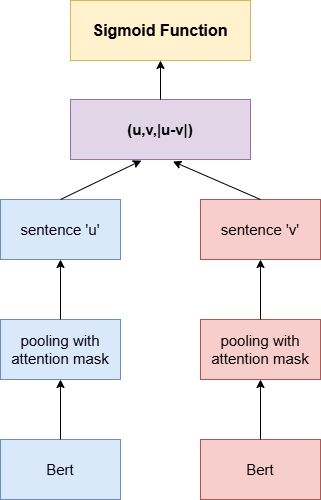
\includegraphics[width=0.6\linewidth]{Figures/SBERT_PD.png}
    \caption{SBERT Implementation Architecture for Paraphrase Detection. Referenced from \textit{Sentence-BERT: Sentence Embeddings using Siamese BERT-Networks} by Reimers and Gurevych~\cite{reimers2019sentence}}
    \label{fig:sbert_pd_architecture}
\end{figure}

\subsection{Semantic Textual Similarity (Regression Task)}

\textbf{Objective:} Estimate a continuous similarity score (0 to 5) that reflects how semantically close two sentences are.

\textbf{Embedding Interaction:} Sentence embeddings $u$ and $v$ are obtained using MEAN pooling and attention masking, as in the classification task.

\textbf{Similarity Computation:} Cosine similarity is computed between the two vectors:
\[
\text{sim}(u, v) = \frac{u^\top v}{\|u\| \cdot \|v\|}
\]
To match the STSb dataset scale (0 to 5), we use:
\[
\text{similarity} = \text{sim}(u, v) \times 2.5 + 2.5
\]

\textbf{Loss Function:} Mean Squared Error (MSE) loss is employed during training for this task:
\[
\mathcal{L}_{\text{regression}} = \frac{1}{N} \sum_{i=1}^{N} (s_i - \hat{s}_i)^2
\]
Where $s_i$ is the ground truth similarity score and $\hat{s}_i$ is the predicted similarity.

\textbf{Evaluation Metric - Pearson Correlation:}
Pearson Correlation measures the linear alignment between predicted and ground truth scores. Formula is
\[
r = \frac{\sum (x_i - \bar{x})(y_i - \bar{y})}{\sqrt{\sum (x_i - \bar{x})^2} \cdot \sqrt{\sum (y_i - \bar{y})^2}}
\]
where \( x_i \) denotes the predicted score, \( \bar{x} \) is the mean of the predicted scores, \( y_i \) is the ground truth score, \( \bar{y} \) is the mean of the ground truth scores, and \( r \) is the Pearson correlation coefficient.

Unlike MSE, Pearson correlation evaluates how well the model preserves the ranking of similarity across examples — which is the actual goal in STS.

\begin{figure}[H]
    \centering
    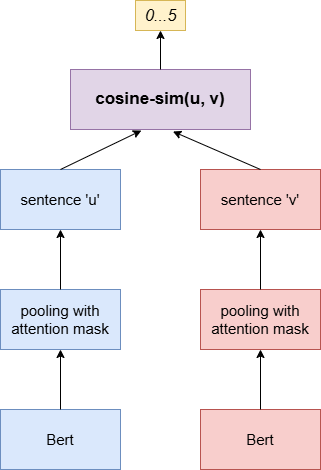
\includegraphics[height=10cm]{Figures/SBERT_STS.png}
    \caption{SBERT Implementation Architecture for Semantic Textual Similarity. Referenced from \textit{Sentence-BERT: Sentence Embeddings using Siamese BERT-Networks} by Reimers and Gurevych~\cite{reimers2019sentence}}
    \label{fig:sbert_sts_architecture}
\end{figure}

\subsection{Training Details}
The paraphrase detection model is trained using the QQP dataset with sigmoid activation and Binary Cross Entropy loss. The STS model is trained using the STSb dataset with cosine similarity and MSE loss. Dropout regularization is applied after pooling to prevent overfitting. Attention masking is consistently used to exclude padding tokens during pooling. Fine-tuning parameters such as learning rate and batch size are selected empirically to optimize performance.